\documentclass[12pt]{article} 

\usepackage{amsmath}
\usepackage{amssymb}
\usepackage{graphicx}
\usepackage{subfigure}


\usepackage[left=2cm,right=2cm,bottom=2cm,top=2cm]{geometry}

\title{
  CreateSkin: Generating a trace of the sphere motion.
}

\author{ Volodymyr Sergiievskyi}


\begin{document}

\maketitle

\section{Task}
A 3d Euclidean point cloud aligned in main axis directions (x, y, z) and with a constant distance grid starting at a given reference point (the point with indices 0, 0, 0 is located at reference point) is intersected by a move of sphere,
 where the path of the sphere center is defined by a user given formula $x = f (t)$ where $t$ is in the interval between $t_0$ and $t_1$ . 
 
 The function $f(t)$ can
be handled as a discrete function with a user given $\Delta t$.
 Points that intersect with the sphere move are considered as deleted.


 Only the first layer of points (which remains visible/undeleted) from top view must be written
to a file as ASCII data (the skin of the point cloud from top view). The file
format is defined as follows:

\begin{itemize}
  \item Each line contains a single point.
  \item The point definition contains x, y and z coordinates delimited by space characters.
  \item Each line ends with a new line character.
\end{itemize}

%%%%%%%%%%%%%%%%%%%%%%%%%%%%%%%%%%%%%
\section{Skin of the point cloud}
%%%%%%%%%%%%%%%%%%%%%%%%%%%%%%%%%%%%


The point cloud can be implemented as the 3d-array of booleans of size $n_x \times n_y \times n_z$, where the element $(i,j,k)$ corresponds to the point 
$
  \mathbf p = ( x_0 + i \cdot \Delta x , y_0 + j \cdot \Delta y, z_0 + \cdot \Delta z ) 
$
where $\mathbf r = (x_0,y_0,z_0) $ is a reference point,
$\Delta x = \Delta y = \Delta z = \Delta $ is a grid spacing.
The value "True" means that the point is in the array, the value "False" means it was cut.

To generate the skin visible from top it is enough to go through all x and y values and for each of them find the highest not-Deleted point in z direction. 
This can be done by going from top to bottom and looking for the first ``True'' value in the 3d array.
This can be implemented by the following algorithm:
\begin{verbatim}
  for(ix=0;ix<nx;ix++)
    for(iy=0; iy<ny;iy++)
      for(iz = nz-1; iz>=0; iz--)
        if( Array[ix][iy][iz] ) { 
           output_point_at(ix,iy,iz); 
           break; 
        }
\end{verbatim}



%%%%%%%%%%%%%%%%%%%%%%%%%%%%%%%%%%%%%%%%%%%%%%%%%%%%%%%%%%
%%%%%%%%%%%%%%%%%%%%%%%%%%%%%%%%%%%%%%%%%%%%%%%%%%%%%%%%%%
\section{Spherical cut}
%%%%%%%%%%%%%%%%%%%%%%%%%%%%%%%%%%%%%%%%%%%%%%%%%%%%%%%%%%
%%%%%%%%%%%%%%%%%%%%%%%%%%%%%%%%%%%%%%%%%%%%%%%%%%%%%%%%%%


%%%%%%%%%%%%%%%%%%%%%%%%%%%%%%%%%%%%%%%%
\subsection{Indicator function}
%%%%%%%%%%%%%%%%%%%%%%%%%%%%%%%%%%%%%%%


The sphere can be viewed as a particular case of 3d-shape.
Any 3d-shape $S$ can be defined as a set of points which belongs to this shape:
\begin{equation}
    S = \{ \mathbf{a} \in \mathbb{R}^3 : P(\mathbf a) \}
\end{equation}
where $P(\mathbf a)$ is the \emph{indicator function}, which is true for the points $\mathbf a$ inside the shape and false otherwise. 
For example, the indicator function of sphere is 
\begin{equation}
  P_{sph}(\mathbf a) \equiv ( | \mathbf a - \mathbf c | < R )
\end{equation}
where $\mathbf c$ is the center of the sphere, and $R$ is the radius. 




\begin{figure}
\subfigure[\label{fig:sphere} Fragment of the point cloud with the cut of spheres ] { 
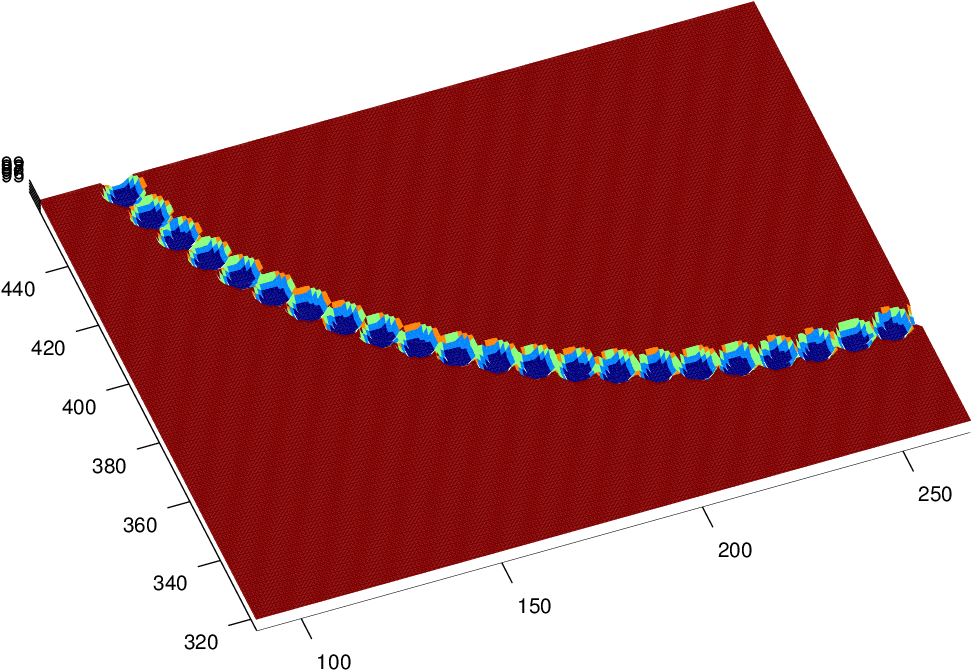
\includegraphics[width=0.5\textwidth]{holes1}
}
\subfigure[\label{fig:cylinder_cut}
Fragment of the point cloud with the cut of spheres and the cylinders connecting their centers
] { 
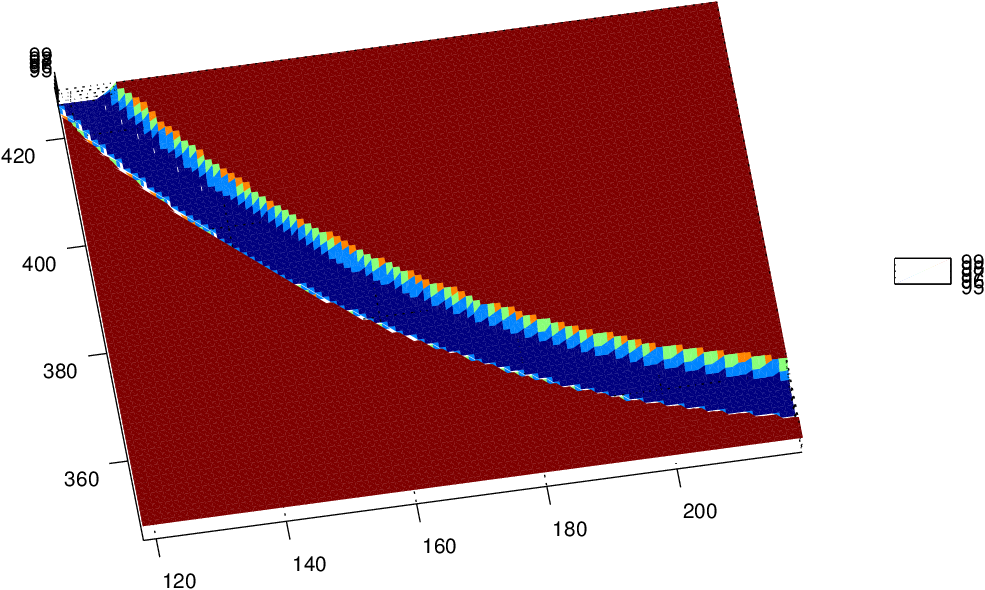
\includegraphics[width=0.5\textwidth]{cylinder_cut1}
}
\caption{Two fragments of the skin demonstrate two methods to cut the points from the point cloud: just cutting the spheres (left) or cutting additionally cylinders which connect their centers (right)}
\end{figure}


\begin{figure}
\subfigure[\label{fig:cyl} To check whether the point P is inside the cylinder we need to check that it lines at the distance less than R from its axis (PQ$<$R) and that the projection Q of P is between the bases of the cylinder (CQ $<$ AC) ] { 
$\qquad$
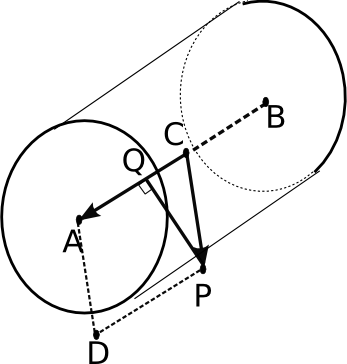
\includegraphics[width=0.3\textwidth]{cyl}
$\qquad$$\qquad$
}
\subfigure[\label{fig:cyl_bounds}
Bounding box of the cylinder can be calculated by taking minimal and maximal coordinates of the centers of the bases (A and B), and increasing the ranges by the radius R from each side
] { 
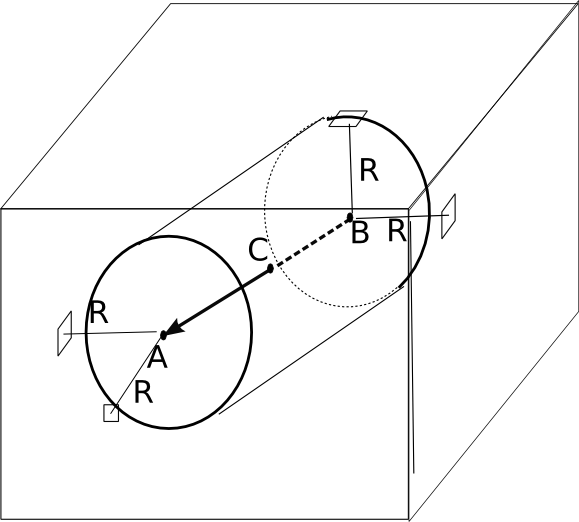
\includegraphics[width=0.5\textwidth]{cyl_bounds}
}
\caption{
Cylinder indicator function and bounding box}
\end{figure}

%%%%%%%%%%%%%%%%%%%%%%%%%%%%%%%%%%%%%%%%%%%%%%%
\subsection{Bounding Box}
%%%%%%%%%%%%%%%%%%%%%%%%%%%%%%%%%%%%%%%%%%%%%%%%%%

The simplest way to cut the shape out the point cloud we can easily go through the all points of the cloud, check for each of them the indicator function $P(\mathbf a)$ and if it is true, change the corresponding values in the 3d-array representing cloud to "False" (which means to remove the point).
However, this approach would need $n_x \times n_y \times n_z$ operations, which can be a big number if the dimensions are large.
However, to accelerate the calculations we can exclude from the consideration the points which are obviously not in the shape. 
To do this, we can define a \emph{bounding box} $B$ of the shape, which is the cuboid which contains the shape, i.e:
\[
  B = [x_1; x_2 ]\times [y_1; y_2]\times [z_1; z_2] : 
\]  
\[ 
    \forall \mathbf{a} = (x,y,z) \notin B \text{~is true~}    \mathbf a \notin S  ( \text{~or~} P(\mathbf a) = \text{~False} )
\]
For example, the bounding box for sphere can be defined as 
\[
   B = [x_c - R; x_c + R] \times [y_c - R; y_c + R] \times [z_c-R; z_c+R]
\]
where $\mathbf c = (x_c,y_c,z_c)$ is the center of the sphere, $R$ is the radius.

This allows us to consider only a subset of points namely points with indices 
from $(x_1 - x_0)/\Delta$ to $(x_2-x_0)/\Delta$, 
from $(y_1 - y_0)/\Delta$ to $(y_2-y_0)/\Delta$ 
and from $(z_1 - z_0)/\Delta$ to $(z_2-z_0)/\Delta$ in $x$,$y$ and $z$ directions correspondingly. 

The described above approach was used to cut the spheres which lies along the circular trajectory. One can see the results in Figure \ref{fig:sphere}.


%%%%%%%%%%%%%%%%%%%%%%%%%%%%%%%%%%%%%%%%%%%%%%%%%%%%%%%%%%%%%%%
%%%%%%%%%%%%%%%%%%%%%%%%%%%%%%%%%%%%%%%%%%%%%%%%%%%%%%%%%%%%%%%
\section{Cylindrical cut}
%%%%%%%%%%%%%%%%%%%%%%%%%%%%%%%%%%%%%%%%%%%%%%%%%%%%%%%%%%%%%%%
%%%%%%%%%%%%%%%%%%%%%%%%%%%%%%%%%%%%%%%%%%%%%%%%%%%%%%%%%%%%%%%


%%%%%%%%%%%%%%%%%%%%%%%%%%%%%%%%%%%%%%%%%%%%%%%%%%%%%
\subsection{Problems of the spherical cut}
%%%%%%%%%%%%%%%%%%%%%%%%%%%%%%%%%%%%%%%%%%%%%%%%%%%%


After the close view on the spherical cut shown in Figure \ref{fig:sphere} we see, that the cut is not smooth, so the traces of individual spheres are clearly seen.
To improve the situation we can, of course, reduce the parameter step of the function used to get the sphere centers.
However, this will significantly increase the computational effort. 
Another approach would be just to cut additionally to the spheres the cylinders of radius $R$ which connect the centers of the spheres at two sequential trajectory points.
In order to be able to do this according to the previously described algorithm we need to define the indicator function and the bounding box of a cylinder.

%%%%%%%%%%%%%%%%%%%%%%%%%%%%%%%%%%%%%%%%%%%%%%%%%%%%%%%%%%
\subsection{Indicator function of a cylinder }
%%%%%%%%%%%%%%%%%%%%%%%%%%%%%%%%%%%%%%%%%%%%%%%%%%%%%%%%
We define a cylinder by its the radius $R$, its center $C$ and the vector $CA$ which connects the center of the cylinder with the center $A$ of one of the bases (see Figure \ref{fig:cyl} ).
The center of the second base we refer as $B$.
Let the point P is given and we want to test weather it lies inside the cylinder or not.
In order to do it, we need to test two conditions:
 \begin{enumerate}
   \item The distance PQ from the point to the axis $\vec{AB}$ is smaller than the radius R.
   \item The projection $Q$ of the point $P$ to the axis lies between the centers of the bases of the cylinder.
 \end{enumerate}
 
%------------------------------------------------------------------ 
 \subsubsection*{Distance from point to the axis of cylinder}
%------------------------------------------------------------------ 
 
    To calculate the distance to the axis we use the fact that the absolute value  of vector product $|[\vec{CP} \times \vec{CA}]|$ is equal to the area of parallelogram CPDA. 
    From the other side  the area of the parallelogram is a product of the base by the height, i.e:
    \[
     S_{CPDA} = |\vec{CA}| \cdot h ~~~ \Rightarrow ~~~ h =  |\vec{PQ}| = { | \vec{CP} \times \vec{CA} | \over |\vec{CA}| }         
   \]  
    It should hold $h<R$, i.e. the condition to check is:
 \[
   { | \vec{CP} \times \vec{CA}| \over |\vec{CA}| } < R
 \]

%-------------------------------------------------------------     
  \subsubsection*{Check if the point is between the bases}     
%------------------------------------------------------------  
  
       To check whether the point is between the bases of the cylinder,   we need to ensure  that projection $Q$ of the point $P$ on the axis AB lies between A and B.
      This holds in case if $|\vec{CQ}| < |\vec{CA}|$.
      To calculate the projection we divide the scalar product 
      $\vec{CP} \bullet \vec{CA}$ by the length of $\vec{CA}$:
       \[
           \vec{CQ} = { \vec{CP} \bullet \vec{CA} \over |\vec{CA}| }
        \]

 So summarizing the two conditions we can write the indicator function of the cylinder in a following way:
 
 \[
    P_{cyl}(\mathbf{P}) \equiv 
      \left(  
          {|\vec{CP} \times \vec{CA}| \over |\vec{CA}|  }  < R 
     \right)
        \land
     \left(  
         { | \vec{CP} \bullet \vec{CA} | \over |\vec{CA}|  }  < |\vec{CA}| 
     \right)
 \]


%%%%%%%%%%%%%%%%%%%%%%%%%%%%%%%%%%%%%%%%%%%%%%%%%%%%%%%%%%%%%%%
\subsection{Bounding box of a cylinder}
%%%%%%%%%%%%%%%%%%%%%%%%%%%%%%%%%%%%%%%%%%%%%%%%%%%%%%%%%%%%%%%

The bounding box of the cylinder can be taken just as the box, which contains the axis (AB), enlarged by the radius $R$ in each direction 
(see Figure \ref{fig:cyl_bounds}):
\[
   B_{cyl} = [x_1-R;x_2+R] \times [y1-R; y_2+R] \times [z_1-R; z_2+R]
\]
where 
$$ x_1 = \min(x_A,x_B)  \qquad  x_2 = \max(x_A,x_B)  $$
\[ y_1 = \min(y_A,y_B)  \qquad  y_2 = \max(y_A,y_B)  \]
\[ z_1 = \min(z_A,z_B)  \qquad  z_2 = \max(z_A,z_B)  \]
\[  A = (x_A,y_A,z_A)  \]
\[  B = (x_B,y_B,z_B)  \]

This method is consistent, in a sense that the bounding box contains all the points of the cylinder:
\[
   \forall \mathbf a : P_{cyl}(\mathbf a) \Rightarrow \mathbf a \in B_{cyl}
\]
It is true, that the bounding box defined in such a way is not minimal, i.e. there can exist a smaller box which also contains all the points of the cylinder. 
However, not minimality is not that crucial in our case, because we use the bounding box only for acceleration of calculations.
This means that with any consistent definition of the bounding box we would get a correct result, while not minimal boxes will need a little bit more computational time.
So, for the sake of simplicity we leave the current definition and use it in the code, but have in mind that it can be improved in future.

%%%%%%%%%%%%%%%%%%%%%%%%%%%%%%%%%%%%%%%%%%%%%%%%%%%%%%%%%%
%%%%%%%%%%%%%%%%%%%%%%%%%%%%%%%%%%%%%%%%%%%%%%%%%%%%%%%%%%
\section{Results}
%%%%%%%%%%%%%%%%%%%%%%%%%%%%%%%%%%%%%%%%%%%%%%%%%%%%%%%%%%
%%%%%%%%%%%%%%%%%%%%%%%%%%%%%%%%%%%%%%%%%%%%%%%%%%%%%%%%%%

Having the indicator function and the bounding box of a cylinder it is possible to cut the cylinders which connect the successive point on the sphere's trajectory. 
The results one can see in Figure \ref{fig:cylinder_cut}.
We see a big improvement in comparison to the previous method of spherical cut (Figure \ref{fig:sphere}), while the computation time is comparable in both cases. 













\end{document}
